\documentclass{article}
\usepackage{amsmath, amssymb, tcolorbox, array, sfmath, enumerate, multicol, pgfplots}
\renewcommand{\familydefault}{\sfdefault}
\pgfplotsset{compat=newest}
\usetikzlibrary{arrows.meta}
\everymath{\displaystyle}
\tikzset{>=stealth}
\tikzstyle{input} = [circle, text centered, radius = 1cm, draw = black]
\tikzstyle{function} = [rectangle, text centered, minimum width = 2cm, minimum height = 1cm, draw = black]
\usepackage[top = 0.25in, bottom = 0.25in, left = 1in, right = 1in]{geometry}
\pagestyle{empty}
\raggedright

\newcounter{example}[section]
\newenvironment{example}[1][]{\refstepcounter{example}\par\medskip
   {\color{red}\textbf{Example~\theexample. #1}}}{\medskip}

\begin{document}

\section*{Absolute Value Equations}

\begin{tcolorbox}[colframe=orange!70!white, coltitle=black, title=\textbf{Summary}]
\begin{enumerate}
    \item You will \emph{usually} have 2 solutions to absolute value equations.
\end{enumerate}
\end{tcolorbox}
\bigskip 

The {\color{blue}\textbf{absolute value}} of a number, $b$, denoted $|b|$, is the distance $b$ is from 0 on a number line.	
\bigskip 

For $|x| = 2$, we get two possible values for $x$: \quad 2 and $-2$		\newline\\	

\begin{center}
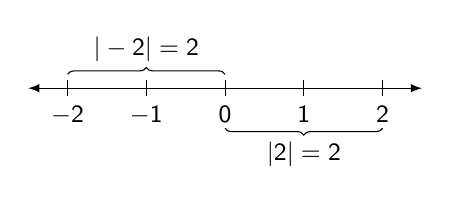
\begin{tikzpicture}
	\draw [<->, > = latex] (-2.5,0) -- (2.5,0);
	\foreach \x in {-2,-1,0,1,2}
	\draw (\x, -0.1) -- (\x, 0.1);
	\foreach \x in {-2,-1,0,1,2}
	\node at (\x, -0.1) [below] {\small $\x$};
	\draw[decoration={brace, raise=5pt},decorate] (-2,0) -- node[above=6pt] {\small $|-2|=2$} (0,0);
	\draw[decoration={brace, mirror, raise=0.2in},decorate] (0,0) -- node[below=0.22in] {\small $|2|=2$} (2,0);
\end{tikzpicture}
\end{center}
\vspace{0.25in}

\begin{center}
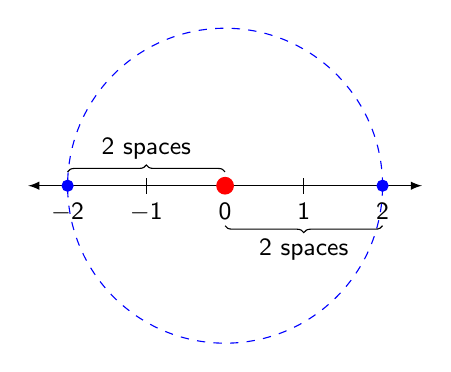
\begin{tikzpicture}
	\draw [<->, > = latex] (-2.5,0) -- (2.5,0);
	\foreach \x in {-2,-1,0,1,2}
	\draw (\x, -0.1) -- (\x, 0.1);
	\foreach \x in {-2,-1,0,1,2}
	\node at (\x, -0.1) [below] {\small $\x$};
    \draw [red, fill=red] (0,0) circle [radius = 3pt];
    \draw [blue, dashed] (0,0) circle [radius = 2cm];
    \draw [blue, fill=blue] (-2,0) circle [radius = 2pt];
    \draw [blue, fill=blue] (2,0) circle [radius = 2pt];
    \draw[decoration={brace, raise=5pt},decorate] (-2,0) -- node[above=6pt] {\small 2 spaces} (0,0);
	\draw[decoration={brace, mirror, raise=0.2in},decorate] (0,0) -- node[below=0.22in] {\small 2 spaces} (2,0);
\end{tikzpicture}
\end{center}
\bigskip 

When solving absolute value equations:

\begin{itemize}
    \item $[|x| = c \text{ means that } x=c \text{ or } x=-c$.
    \item Isolate your absolute value bars on one side (if possible) \underline{before} separating into 2 equations.
    \item Check your answers in the \emph{original problem}.
\end{itemize}
\bigskip 

\begin{example}
Solve each.
\begin{enumerate}[(a)]
\begin{multicols}{3}
    \item $|2x-3| = 11$ 
    \item $|3x-1| = 5$ 
    \item $|x+5| = 2x$
\end{multicols}
\vfill 
\newpage 
\begin{multicols}{2}
    \item $|4x-3| = 5x + 1$
    \item $|x+1| = -2$ 
\end{multicols}
\vfill 
\begin{multicols}{2}
    \item $|-x+2|-4 = 10$
    \item $|3x-1| = |x+5|$
\end{multicols}
\end{enumerate}
\end{example}
\vfill 

\end{document}
